% ===================================================================
%  Week 2 — Lecture Notes (Persian) — Point Operations & Histograms
%  Compile: xelatex -interaction=nonstopmode notes.tex   (twice)
% ===================================================================
\documentclass[12pt,a4paper]{article}
% ===================================================================
%  Shared preamble for Persian lecture notes (Image Processing).
%  Compile with XeLaTeX.  Body = Persian (RTL), code/math = LTR.
% ===================================================================

\usepackage{geometry}
\geometry{a4paper,margin=2.4cm}
\usepackage{amsmath,amssymb}
\usepackage{graphicx}
\usepackage{xcolor}
\usepackage{listings}
\usepackage{tcolorbox}
\usepackage{booktabs}
\usepackage{array}
\usepackage{enumitem}
\usepackage{hyperref}
\tcbuselibrary{skins,breakable}

% ---- Persian / RTL --------------------------------------------------
\usepackage{xepersian}
\settextfont{IRNazli}
\setlatintextfont{Latin Modern Roman}
\setdigitfont{IRNazli}
% More generous leading + paragraph spacing (Persian reads better with air).
\linespread{1.5}
\setlength{\parskip}{0.7em}

% ---- Colours --------------------------------------------------------
\definecolor{coursePrimary}{HTML}{1B4965}
\definecolor{courseAccent}{HTML}{E76F51}
\definecolor{courseGood}{HTML}{2A9D8F}
\definecolor{courseBad}{HTML}{C0392B}
\definecolor{courseInfo}{HTML}{2980B9}
\definecolor{codeBg}{HTML}{F5F6FA}
\definecolor{codeKw}{HTML}{8E44AD}
\definecolor{codeStr}{HTML}{2A9D8F}
\definecolor{codeCom}{HTML}{7F8C8D}

\hypersetup{colorlinks=true,linkcolor=courseInfo,urlcolor=courseInfo,citecolor=courseInfo}

% ---- Code listings (Python built in) -------------------------------
\lstdefinestyle{course}{
  backgroundcolor=\color{codeBg},
  basicstyle=\ttfamily\small,
  keywordstyle=\color{codeKw}\bfseries,
  stringstyle=\color{codeStr},
  commentstyle=\color{codeCom}\itshape,
  numberstyle=\tiny\color{codeCom},
  numbers=left, numbersep=7pt,
  showstringspaces=false, breaklines=true,
  tabsize=4, columns=fullflexible, frame=single,
  rulecolor=\color{gray!30}, keepspaces=true, upquote=true, language=Python,
}
\lstset{style=course}
\lstdefinelanguage{bash}{
  keywords={cd,pip,python,venv,source,import}, sensitive=true,
  morecomment=[l]{\#}, morestring=[b]', morestring=[b]",
}
\newenvironment{ltrcode}{\begin{LTR}}{\end{LTR}}

% ---- Callout boxes (Persian titles) --------------------------------
\newtcolorbox{yaddasht}{colback=courseInfo!8,colframe=courseInfo,
  title={\textbf{یادداشت}},boxrule=0.6pt,right=6pt,left=6pt,breakable}
\newtcolorbox{nokte}{colback=courseAccent!10,colframe=courseAccent,
  title={\textbf{نکتهٔ کلیدی}},boxrule=0.6pt,right=6pt,left=6pt,breakable}
\newtcolorbox{hoshdar}{colback=courseBad!8,colframe=courseBad,
  title={\textbf{هشدار / دام}},boxrule=0.6pt,right=6pt,left=6pt,breakable}
\newtcolorbox{riyazi}{colback=coursePrimary!6,colframe=coursePrimary,
  title={\textbf{ریاضیات}},boxrule=0.6pt,right=6pt,left=6pt,breakable}
\newtcolorbox{tamrin}{colback=courseGood!8,colframe=courseGood,
  title={\textbf{تمرین}},boxrule=0.6pt,right=6pt,left=6pt,breakable}

% ---- Header helper --------------------------------------------------
\newcommand{\coursemeta}[2]{%
  \begin{center}
  {\large\textbf{پردازش تصویرِ کاربردی}}\\[2pt]
  {\color{coursePrimary}\rule{\linewidth}{1pt}}\\[4pt]
  {\Large\textbf{#1}}\\[3pt]
  {\small جزوهٔ درس — #2}
  \end{center}\vspace{4pt}
}


\begin{document}
\coursemeta{جلسهٔ ۲ — عملیاتِ نقطه‌ای و هیستوگرام}{هفتهٔ دوم}

{\small\itshape مکملِ اسلایدهای انگلیسیِ جلسهٔ ۲. همهٔ تصاویرِ این جزوه از دیتاستِ واقعیِ شما (کنتورِ آب در \lr{E:/data}) تولید شده‌اند. هدف: تشخیصِ نوردهی/کنتراست از روی هیستوگرام و اصلاحِ آن.}

\vspace{0.5cm}
\tableofcontents
\vspace{1cm}

% ===================================================================
\section{چرا این جلسه}

عکس‌های کنتورِ DocScan اغلب تاریک یا کم‌کنتراست‌اند. اصلاحِ نوردهی، اولین گام برای خواندنِ ارقام
است. امروز \textbf{عملیاتِ نقطه‌ای} (که هر پیکسل را مستقل تبدیل می‌کند) و \textbf{هیستوگرام} (ابزاری
که می‌گوید چه تبدیلی لازم است) را یاد می‌گیریم.

\subsection{دو خانوادهٔ عملیات}

پردازش‌های تصویر را می‌توان به دو خانوادهٔ بزرگ تقسیم کرد که در کلِ کورس بارها می‌بینیم:

\begin{itemize}
  \item \textbf{عملیاتِ نقطه‌ای} (این جلسه): خروجیِ هر پیکسل فقط به \emph{ورودیِ همان پیکسل} بستگی
        دارد. سریع، ساده، برای نوردهی/کنتراست.
  \item \textbf{عملیاتِ همسایگی} (جلسات ۳ به بعد): خروجیِ هر پیکسل به \emph{پنجره‌ای از پیکسل‌های
        اطراف} بستگی دارد. برای تاری، تیزی، لبه، نویز.
\end{itemize}

این تقسیم‌بندیِ ذهنی مهم است: وقتی با یک مسئله روبه‌رو می‌شوید، اول بپرسید «آیا این با نگاه به تکِ
پیکسل حل می‌شود، یا به همسایه‌ها نیاز دارم؟» — پاسخ، خانوادهٔ ابزارِ درست را مشخص می‌کند.

% ===================================================================
\section{هیستوگرام: سرشماریِ روشنایی}

\textbf{هیستوگرام} یک تصویر می‌شمارد چند پیکسل هر سطحِ روشنایی (۰ تا ۲۵۵) را دارند. محورِ افقی
شدت، محورِ عمودی تعداد. یک نمای کنتورِ واقعی و هیستوگرامش:

\begin{center}
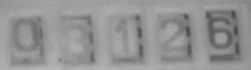
\includegraphics[width=0.5\linewidth]{../assets/gray.png}\\[3pt]
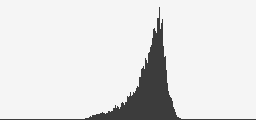
\includegraphics[width=0.5\linewidth]{../assets/hist_before.png}\\[2pt]
{\small تصویرِ خاکستری (بالا) و هیستوگرامِ آن (پایین) — فشرده، یعنی کم‌کنتراست}
\end{center}

\begin{nokte}
هیستوگرام \emph{کجاییِ} پیکسل‌ها را دور می‌ریزد و فقط \emph{چندتاییِ} هر مقدار را نگه می‌دارد.
دقیقاً همان چیزی که برای استدلال دربارهٔ نوردهی و کنتراست لازم دارید. \emph{اول} هیستوگرام را
بخوانید، بعد به تصویر دست بزنید.
\end{nokte}

\subsection{خواندنِ هیستوگرام}

\begin{itemize}
  \item پیک در \textbf{چپ} = تاریک (کم‌نور). در \textbf{راست} = روشن (پرنور).
  \item \textbf{باریک} = کم‌کنتراست. \textbf{پخش‌شده در کلِ بازه} = کنتراستِ خوب.
  \item دو پیک (\textbf{دوقله‌ای}، \lr{bimodal}) = شیء در برابرِ پس‌زمینه — هدیه‌ای برای آستانه‌گذاری.
\end{itemize}

\begin{ltrcode}
\begin{lstlisting}[language=Python]
import cv2, numpy as np
gray = cv2.cvtColor(cv2.imread('E:/data/abfa_image/numerators/num_3494.jpg'),
                    cv2.COLOR_BGR2GRAY)
hist = cv2.calcHist([gray], [0], None, [256], [0, 256])   # 256 bins
print(gray.min(), gray.max(), gray.mean())    # quick exposure check
\end{lstlisting}
\end{ltrcode}

% ===================================================================
\section{عملیاتِ نقطه‌ای}

یک \textbf{عملیاتِ نقطه‌ای} مقدارِ هر پیکسل را از یک تابعِ $s = T(r)$ عبور می‌دهد — مستقل از
همسایه‌ها. روشنایی: $s = r + b$. کنتراست: $s = a\cdot r$. منفی: $s = 255 - r$. با یک
\textbf{جدولِ جست‌وجو} (\lr{LUT}) پیاده می‌شود: $T$ را یک‌بار برای ۰ تا ۲۵۵ حساب کنید و سریع
روی همهٔ پیکسل‌ها اعمال کنید.

\begin{riyazi}
خطیِ عمومی: $s = a\cdot r + b$ — $a$ کنتراست را مقیاس می‌دهد، $b$ روشنایی را جابه‌جا می‌کند.
سپس به ۰ تا ۲۵۵ \lr{clip} کنید.
\end{riyazi}

\subsection{تصحیحِ گاما — روی کنتورِ واقعی}

\begin{center}
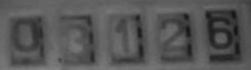
\includegraphics[width=0.3\linewidth]{../assets/gamma_dark.png}\quad
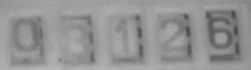
\includegraphics[width=0.3\linewidth]{../assets/gray.png}\quad
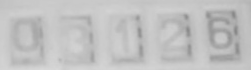
\includegraphics[width=0.3\linewidth]{../assets/gamma_bright.png}\\[2pt]
{\small چپ: $\gamma<1$ (تاریک‌تر) — وسط: اصلی — راست: $\gamma>1$ (روشن‌تر)}
\end{center}

\begin{riyazi}
$s = 255\,(r/255)^{1/\gamma}$ — یک منحنیِ \emph{غیرخطی} که سایه‌ها را روشن می‌کند بدونِ
سوزاندنِ های‌لایت‌ها.
\end{riyazi}

خطی ($ar+b$) همه‌چیز را یکسان جابه‌جا/مقیاس می‌کند — می‌تواند های‌لایت را ببُرد یا سایه را له کند.
گاما \textbf{غیرخطی} است: تُن‌های تاریک را بیشتر از روشن بالا می‌برد. برای یک عکسِ کنتورِ تاریک،
گاما اغلب ارقامی را بازمی‌گرداند که روشن‌سازیِ خطی آن‌ها را می‌شست.

\begin{nokte}
ابزار را با هیستوگرام تطبیق دهید: جابه‌جا-اما-پخش $\rightarrow$ روشنایی؛ فشرده $\rightarrow$
کنتراست/گاما. این تشخیص، تفاوتِ اصلاحِ هدفمند و آزمون‌وخطای کور است.
\end{nokte}

% ===================================================================
\section{تبدیل‌های نقطه‌ایِ دیگر}

\subsection{تصویرِ منفی}

$s = 255 - r$ روشن را تاریک و تاریک را روشن می‌کند. مفید برای دیدنِ جزئیات در نواحیِ تیره (مثلِ
عکسِ رادیولوژی) یا وقتی متن روشن روی زمینهٔ تیره است و می‌خواهید معکوسش کنید.

\subsection{تبدیلِ لگاریتمی}

\begin{riyazi}
$s = c \cdot \log(1 + r)$ — تُن‌های تاریک را زیاد می‌کشد و روشن‌ها را فشرده می‌کند.
\end{riyazi}

مفید وقتی بازهٔ دینامیکی خیلی زیاد است (مثلِ طیفِ فوریه در جلسهٔ ۶، که مقادیرش ده‌ها مرتبهٔ بزرگی
تفاوت دارند و بدونِ لگاریتم اصلاً دیدنی نیستند). تبدیلِ \textbf{نمایی/توانی} (همان گاما) عکسِ این
اثر را دارد.

\subsection{برش‌دهیِ شدت (Intensity slicing)}

گاهی فقط یک \emph{بازهٔ} خاصِ شدت مهم است. برش‌دهی، پیکسل‌های آن بازه را برجسته (مثلاً سفید) و بقیه
را سرکوب می‌کند. مثالِ عملی: در یک کنتور، اگر ارقام در بازهٔ شدتِ مشخصی باشند، برش‌دهی می‌تواند فقط
آن‌ها را جدا کند — یک آستانه‌گذاریِ دوطرفه.

\begin{ltrcode}
\begin{lstlisting}[language=Python]
mask = ((gray >= 60) & (gray <= 120)).astype(np.uint8) * 255  # keep a band
\end{lstlisting}
\end{ltrcode}

\begin{yaddasht}
همهٔ این‌ها LUT‌اند: یک تابع روی ۰ تا ۲۵۵ که یک‌بار حساب و سریع اعمال می‌شود. وقتی یک تبدیلِ
نقطه‌ایِ جدید نیاز دارید، فقط تابعش را روی ۲۵۶ مقدار تعریف کنید و با \lr{cv2.LUT} اعمال کنید.
\end{yaddasht}

% ===================================================================
\section{بهبودِ کنتراست}

\subsection{کشِ کنتراست (کمینه--بیشینه)}

بازهٔ واقعیِ $[\min,\max]$ را به کلِ $[0,255]$ نگاشت کنید. ساده، برگشت‌پذیر، و نمی‌تواند جزئیات
بسازد — فقط از کلِ بازه استفاده می‌کند.

\begin{center}
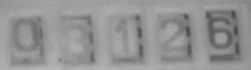
\includegraphics[width=0.42\linewidth]{../assets/gray.png}\quad
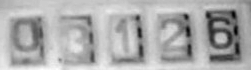
\includegraphics[width=0.42\linewidth]{../assets/stretch.png}\\[2pt]
{\small قبل (چپ) و بعد از کشِ کنتراست به ۰ تا ۲۵۵ (راست)}
\end{center}

\begin{riyazi}
$s = 255\dfrac{r-\min}{\max-\min}$
\end{riyazi}

\subsection{یکسان‌سازیِ هیستوگرام (Histogram Equalization)}

شدت‌ها را بازتوزیع می‌کند تا هیستوگرام (تقریباً) \textbf{یکنواخت} شود. از هیستوگرامِ تجمعی
(\lr{CDF}) به‌عنوانِ تابعِ نگاشت استفاده می‌کند. برای آشکارکردنِ جزئیات در تصاویرِ کم‌کنتراست عالی
است — اما می‌تواند نویز را بیش‌ازحد تقویت کند.

\begin{center}
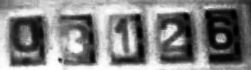
\includegraphics[width=0.42\linewidth]{../assets/equalized.png}\quad
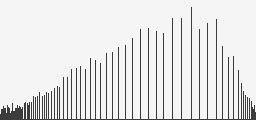
\includegraphics[width=0.42\linewidth]{../assets/hist_after.png}\\[2pt]
{\small کنتورِ یکسان‌سازی‌شده (چپ) و هیستوگرامِ پخش‌شدهٔ آن (راست)}
\end{center}

\begin{ltrcode}
\begin{lstlisting}[language=Python]
stretch   = cv2.normalize(gray, None, 0, 255, cv2.NORM_MINMAX)
equalized = cv2.equalizeHist(gray)
lut       = np.array([((i/255)**(1/0.5))*255 for i in range(256)], np.uint8)
gamma     = cv2.LUT(gray, lut)             # gamma = 0.5
\end{lstlisting}
\end{ltrcode}

\lr{cv2.LUT} یک جدولِ ۲۵۶ درایه‌ای را در یک عبورِ سریع روی هر پیکسل اعمال می‌کند — الگوی هر
عملیاتِ نقطه‌ای.

% ===================================================================
\section{ریاضیاتِ یکسان‌سازیِ هیستوگرام}

چرا یکسان‌سازی کار می‌کند؟ ایدهٔ کلیدی: تابعِ نگاشتی که یک توزیعِ دلخواه را به یکنواخت تبدیل
می‌کند، همان \textbf{تابعِ توزیعِ تجمعیِ} (\lr{CDF}) خودِ توزیع است.

\begin{riyazi}
هیستوگرامِ نرمال‌شده $p(r) = n_r / N$ (نسبتِ پیکسل‌های با شدتِ $r$) را در نظر بگیرید. تابعِ نگاشت:
\[
s = T(r) = 255 \cdot \text{CDF}(r) = 255 \sum_{k=0}^{r} p(k)
\]
یعنی هر شدت به تناسبِ «چند پیکسل از آن تاریک‌تر یا برابرند» به یک شدتِ جدید می‌رود.
\end{riyazi}

\textbf{مثالِ عددیِ کوچک:} فرض کنید یک تصویرِ ۳ بیتی (۸ سطح، ۰ تا ۷) با ۶۴ پیکسل داریم که همه در
سطوحِ ۲، ۳، ۴ متمرکزند (کم‌کنتراست). CDF این سطوح را به کلِ بازهٔ ۰ تا ۷ می‌کشد: سطحِ ۲ به نزدیکِ
۰، سطحِ ۴ به نزدیکِ ۷. نتیجه: کنتراست پخش می‌شود. همین منطق برای ۲۵۶ سطح در تصاویرِ ۸ بیتی برقرار است.

\begin{yaddasht}
این توضیح می‌دهد چرا یکسان‌سازی داده‌محور است: نگاشت کاملاً به هیستوگرامِ همان تصویر بستگی دارد.
دو تصویرِ با هیستوگرام‌های متفاوت، نگاشت‌های متفاوت می‌گیرند — که هم قدرت و هم ضعفِ آن است.
\end{yaddasht}

% ===================================================================
\section{انواعِ آستانه‌گذاری}

\lr{OpenCV} چند نوعِ آستانه دارد که هرکدام کاربردِ خود را دارند:

\begin{center}
\begin{tabular}{>{\raggedright\arraybackslash}p{0.3\linewidth} >{\raggedright\arraybackslash}p{0.6\linewidth}}
\toprule
\textbf{نوع} & \textbf{رفتار} \\
\midrule
\lr{THRESH\_BINARY} & بالای $T$ سفید، پایین سیاه (رایج‌ترین) \\
\lr{THRESH\_BINARY\_INV} & برعکس؛ برای متنِ تیره روی زمینهٔ روشن \\
\lr{THRESH\_TRUNC} & بالای $T$ به $T$ محدود، بقیه بی‌تغییر \\
\lr{THRESH\_TOZERO} & پایینِ $T$ صفر، بقیه بی‌تغییر \\
\bottomrule
\end{tabular}
\end{center}

برای ارقامِ کنتور (تیره روی زمینهٔ روشن)، اغلب \lr{THRESH\_BINARY\_INV} می‌خواهید تا ارقام سفید
شوند و پس‌زمینه سیاه — چون مراحلِ بعدی (مورفولوژی، کانتور) روی اشیای \emph{سفید} کار می‌کنند.

\begin{nokte}
یک تصمیمِ ظریف: «جلو‌زمینه» سفید باشد یا سیاه؟ قراردادِ رایج در پردازش تصویر: شیءِ موردِ علاقه
سفید (۲۵۵)، پس‌زمینه سیاه (۰). اگر برعکس شود، عملیاتِ مورفولوژیک و شمارشِ کانتورِ جلسات بعد
معکوس عمل می‌کنند.
\end{nokte}

% ===================================================================
\section{ترکیبِ عملیات در یک خطِ لوله}

قدرتِ واقعی وقتی است که این عملیات را زنجیر کنید. برای DocScan، یک خطِ لولهٔ نمونهٔ بهبود:

\begin{ltrcode}
\begin{lstlisting}[language=Python]
gray  = cv2.cvtColor(img, cv2.COLOR_BGR2GRAY)
clahe = cv2.createCLAHE(clipLimit=2.0, tileGridSize=(8, 8)).apply(gray)
bin_  = cv2.adaptiveThreshold(clahe, 255, cv2.ADAPTIVE_THRESH_GAUSSIAN_C,
                              cv2.THRESH_BINARY_INV, 31, 10)
# next week: smooth/denoise before threshold; later: morphology to clean bin_
\end{lstlisting}
\end{ltrcode}

\begin{yaddasht}
ترتیب مهم است: بهبودِ کنتراست \emph{قبل} از آستانه (تا ارقام از پس‌زمینه جدا شوند)، و پاک‌سازیِ
مورفولوژیک \emph{بعد} از آستانه (جلسهٔ ۷). هر گام ورودیِ گامِ بعد را آماده می‌کند. طراحیِ این
ترتیب، خودِ مهندسیِ پردازش تصویر است.
\end{yaddasht}

% ===================================================================
\section{تمرینِ کلاسیِ وسط‌جلسه (۱۰ دقیقه)}

\begin{tamrin}
سه عکسِ کنتور به شما داده شده. هیستوگرام‌هایشان: (۱) یک پیکِ بلند نزدیکِ صفر، هیچ‌چیز بالای ۸۰؛
(۲) دو قلهٔ جدا، یکی نزدیکِ ۴۰ و یکی نزدیکِ ۲۱۰؛ (۳) پخشِ نرم از ۰ تا ۲۵۵. برای هرکدام:
کم‌نور/پرنور/کم‌کنتراست است یا خوب؟ چه عملیاتی اعمال می‌کنید و کدام به هیچ بهبودی نیاز \emph{ندارد}؟
کدام آسان‌ترین برای آستانه‌گذاری است و چرا؟
\end{tamrin}

\textbf{جمع‌بندی:} (۱) کم‌نور و کم‌کنتراست $\rightarrow$ گاما ($\gamma<1$) یا کش؛ ارقام در تاریکی
پنهان‌اند. (۲) دوقله‌ای $\rightarrow$ از پیش جداشدنی؛ \emph{ایده‌آل} برای آستانه‌گذاری (شیء در
برابرِ پس‌زمینه). (۳) خوش‌نوردهی، بازهٔ کامل $\rightarrow$ رهایش کنید؛ بهبود ممکن است فقط نویز را
تقویت کند. هیستوگرام می‌گوید \emph{آیا} و \emph{کدام} بهبود — پیش از هر آزمایش.

% ===================================================================
\section{آستانه‌گذاری}

\textbf{آستانه‌گذاری} شدت را به دو کلاس تبدیل می‌کند: $s = 255$ اگر $r>T$ وگرنه $0$. خاکستری را
به سیاه/سفید بدل می‌کند. کلِ بازی، انتخابِ $T$ است. یک هیستوگرامِ دوقله‌ای این را آسان می‌کند. این
گامِ «تیزکردن»ِ DocScan است — ارقام یک ماسکِ تمیز می‌شوند.

\begin{center}
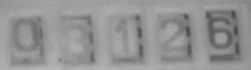
\includegraphics[width=0.42\linewidth]{../assets/gray.png}\quad

\includegraphics[width=0.42\linewidth]{../assets/otsu.png}\\[2pt]
{\small کنتورِ خاکستری (چپ) و آستانهٔ Otsu: ارقام در برابرِ پس‌زمینه (راست)}
\end{center}

\subsection{Otsu: انتخابِ خودکارِ آستانه}

روشِ Otsu آن $T$ را می‌یابد که دو قلهٔ هیستوگرام را بهترین \textbf{جدا} می‌کند. صوری: کمینه‌کردنِ
واریانسِ درون‌کلاسی (معادلِ بیشینه‌کردنِ واریانسِ بین‌کلاسی). یک خط:
\lr{cv2.threshold(g, 0, 255, THRESH\_BINARY+THRESH\_OTSU)}.

\begin{hoshdar}
Otsu دو کلاسِ روشن را فرض می‌کند. روی نورِ ناهموار (سایه‌ای که روی صفحه افتاده) یک $T$ی سراسری
شکست می‌خورد — از آستانه‌گذاریِ \emph{تطبیقی} استفاده کنید.
\end{hoshdar}

\begin{ltrcode}
\begin{lstlisting}[language=Python]
# a local threshold per neighbourhood -> robust to shadows/gradients
binary = cv2.adaptiveThreshold(gray, 255, cv2.ADAPTIVE_THRESH_GAUSSIAN_C,
                               cv2.THRESH_BINARY, blockSize=31, C=10)
\end{lstlisting}
\end{ltrcode}

Otsuِ سراسری برای نورِ یکنواخت؛ تطبیقی برای عکس‌های واقعیِ دارای سایه. عکس‌های DocScan معمولاً به
تطبیقی نیاز دارند.

% ===================================================================
\section{این جلسه در پروژهٔ نهایی (DocScan)}

گامِ «تیزکردن»ِ DocScan (رسیدن به یک تصویرِ باینریِ تمیز از سند/کنتور) مستقیماً از این جلسه
می‌آید. جریانِ عملی برای یک عکسِ کنتور:

\begin{enumerate}
  \item خاکستری کنید و هیستوگرام را ببینید — کم‌کنتراست است؟ سایه دارد؟
  \item بهبود دهید: CLAHE (برای کنتراستِ محلی) یا گاما (اگر تاریک است).
  \item آستانه بزنید: تطبیقی (چون عکسِ موبایل معمولاً نورِ ناهموار دارد).
  \item خروجی: یک ماسکِ باینری که ارقام در آن سفید و پس‌زمینه سیاه است.
\end{enumerate}

این ماسک ورودیِ گام‌های بعدی است: پاک‌سازیِ مورفولوژیک (جلسهٔ ۷)، یافتنِ کانتورِ هر رقم (جلسهٔ ۹)،
و در نهایت شناساییِ رقم با شبکهٔ عصبی (جلسهٔ ۱۳). پس کیفیتِ آستانه‌گذاریِ امروز، مستقیماً دقتِ
خواندنِ نهایی را تعیین می‌کند — یک آستانهٔ بد، ارقام را می‌شکند و OCR شکست می‌خورد.

\begin{yaddasht}
\textbf{مایلستونِ هفتهٔ ۲ برای پروژه:} برای حداقل سه عکسِ کنتورِ سخت، یک تصویرِ باینریِ خوانا از
ارقام تولید کنید و ترکیبِ بهبود+آستانه‌ای را که بهترین کار می‌کند مستند کنید. این پایهٔ کلِ خطِ
لوله است.
\end{yaddasht}

% ===================================================================
\section{بخشِ عمیق}

\subsection{CLAHE: یکسان‌سازیِ محلی و محدود}

یکسان‌سازیِ سراسری در نواحیِ تخت نویز را بیش‌ازحد تقویت می‌کند. \textbf{CLAHE} در کاشی‌های کوچک
یکسان‌سازی می‌کند و هیستوگرام را \textbf{می‌بُرد} تا تقویت را محدود کند. معمولاً پیش‌فرضِ بهتری
برای عکس‌های واقعی است: \lr{cv2.createCLAHE(clipLimit=2.0)}. برای DocScan، CLAHE روی کانالِ
مقدار اغلب از یکسان‌سازیِ ساده بهتر است — کنتراستِ محلی بدونِ انفجارِ نویز.

\subsection{چرا یکسان‌سازی می‌تواند آسیب بزند}

داده‌محور و \textbf{غیرقابلِ‌پیش‌بینی} است: دو تصویرِ مشابه می‌توانند خیلی متفاوت نگاشت شوند. هرچه
هست را تقویت می‌کند — از جمله نویزِ حسگر و بلوک‌های \lr{JPEG}. برای یک خطِ لوله، یک عملیاتِ
\textbf{تعیّنی} (گاما/کشِ ثابت) را ترجیح دهید تا گام‌های بعدی پایدار بمانند.

\begin{nokte}
«برای چشم بهتر به‌نظر می‌رسد» با «برای الگوریتمِ بعدی بهتر است» یکی نیست. برای هدف بهبود دهید، نه
برای دمو. این یکی از مهم‌ترین درس‌های مهندسیِ پردازش تصویر است.
\end{nokte}

\subsection{تطبیقِ هیستوگرام و رنگ}

گاهی می‌خواهید هیستوگرامِ یک تصویر با یک مرجع \emph{تطبیق} کند (ظاهرِ یکنواخت در کلِ دیتاست) —
مفید وقتی عکس‌های کنتور از دوربین‌ها/نورهای مختلف می‌آیند. و برای رنگ: یکسان‌سازیِ جداگانهٔ R، G،
B رنگ را می‌لغزاند (انحرافِ رنگ)؛ به \lr{HSV}/\lr{Lab} بروید، کانالِ \textbf{مقدار/روشنایی} را
بهبود دهید، و برگردید. کنتراستِ جداگانه روی RGB یک اشتباهِ کلاسیکِ تازه‌کار است که کلِ تصویر را
رنگی می‌کند.

% ===================================================================
\section{تنظیمِ پارامترها در عمل}

عملیاتِ نقطه‌ای پارامتر دارند و انتخابشان مهم است. چند راهنمای عملی:

\begin{itemize}
  \item \textbf{گاما}: $\gamma < 1$ تصویر را تاریک‌تر، $\gamma > 1$ روشن‌تر. برای عکسِ کم‌نور معمولاً $\gamma \approx 1.5$ تا $2.5$.
  \item \textbf{آستانهٔ تطبیقی} — \lr{blockSize}: باید فرد و به‌اندازهٔ کافی بزرگ باشد که کلِ یک رقم را در بر بگیرد؛ خیلی کوچک، رقم را تکه‌تکه می‌کند.
  \item \textbf{آستانهٔ تطبیقی} — \lr{C}: از میانگینِ محلی کم می‌شود؛ بزرگ‌ترش نویزِ کمتر ولی خطرِ حذفِ جزئیات.
  \item \textbf{CLAHE} — \lr{clipLimit}: بالاتر یعنی کنتراستِ بیشتر ولی نویزِ بیشتر؛ ۲ تا ۴ متعارف است.
\end{itemize}

\begin{nokte}
هیچ مقدارِ «درست»ِ سراسری وجود ندارد؛ به تصویر بستگی دارد. عادتِ خوب: پارامترها را روی چند
تصویرِ \emph{سخت} (تاریک، سایه‌دار، نویزی) تنظیم کنید، نه روی یک تصویرِ تمیز. پارامتری که فقط روی
تصویرِ آسان کار کند، در عمل شکست می‌خورد.
\end{nokte}

% ===================================================================
\section{چرا عملیاتِ نقطه‌ای کافی نیست}

عملیاتِ نقطه‌ای فقط به \emph{مقدارِ} هر پیکسل نگاه می‌کند، نه به \emph{همسایه‌هایش}. برای همین
نمی‌توانند: تصویر را تار یا تیز کنند، نویز را حذف کنند، یا لبه‌ها را بیابند — چون همهٔ این‌ها به
رابطهٔ یک پیکسل با همسایه‌هایش نیاز دارند. مثال: دو پیکسل با مقدارِ یکسان اما یکی در ناحیهٔ صاف و
دیگری روی یک لبه — عملیاتِ نقطه‌ای نمی‌تواند تفکیکشان کند.

\begin{yaddasht}
اینجا پلی به جلسهٔ ۳ (فیلترِ مکانی و کانولوشن) است: وقتی به همسایه‌ها نیاز داریم، از یک
\textbf{کرنل} استفاده می‌کنیم که روی پنجره‌ای از پیکسل‌ها عمل می‌کند. عملیاتِ نقطه‌ای پایه است؛
فیلترِ مکانی گامِ بعدیِ قدرت.
\end{yaddasht}

% ===================================================================
\section{جمع‌بندی}

\begin{itemize}
  \item خواندنِ هیستوگرام برای تشخیصِ نوردهی و کنتراست.
  \item اعمالِ روشنایی، کنتراست، گاما، کش، یکسان‌سازی — و دانستنِ اینکه کدام مناسب است.
  \item آستانه‌گذاریِ سراسری (Otsu) یا تطبیقی، و دانستنِ اینکه هرکدام کِی شکست می‌خورد.
  \item بهبودِ رنگِ درست (کانالِ مقدار، نه هر RGB).
\end{itemize}

\begin{tamrin}
\textbf{تحویلیِ این هفته (پیش از جلسهٔ ۳):} روی تصاویرِ واقعیِ کنتور/پلاک از \lr{E:/data}:
(۱) هیستوگرام را رسم و نوردهی/کنتراستِ هر تصویر را دسته‌بندی کنید. (۲) کش، یکسان‌سازی، گاما و
CLAHE را اعمال و مقایسه کنید (قبل/بعد). (۳) یک باینریِ تمیزِ Otsu \emph{و} تطبیقی از ارقام
بسازید؛ بگویید کدام برنده است و چرا. (۴) یادداشت: برای تصویرِ DocScanِ شما، کدام ترکیبِ
بهبود+آستانه بهترین خوانایی را می‌دهد؟
\end{tamrin}

\subsection*{دستورالعمل‌های تشخیصی}

\begin{center}
\begin{tabular}{>{\raggedright\arraybackslash}p{0.4\linewidth} >{\raggedright\arraybackslash}p{0.5\linewidth}}
\toprule
\textbf{نشانه (از هیستوگرام/تصویر)} & \textbf{درمان} \\
\midrule
پیک در چپ، تصویر تاریک & گاما $\gamma>1$ یا کشِ کنتراست \\
هیستوگرامِ باریک، کم‌کنتراست & کش یا یکسان‌سازی/CLAHE \\
سایه در بخشی از تصویر & آستانهٔ تطبیقی، نه Otsuِ سراسری \\
دوقله‌ای و واضح & Otsu مستقیم \\
نویز پس از یکسان‌سازی & CLAHE با \lr{clipLimit} پایین \\
انحرافِ رنگ پس از بهبود & روی کانالِ Value کار کنید، نه RGB \\
\bottomrule
\end{tabular}
\end{center}

\subsection*{چک‌لیستِ دام‌های این هفته}

\begin{itemize}
  \item یکسان‌سازیِ جداگانهٔ کانال‌های RGB (انحرافِ رنگ) — به‌جایش کانالِ Value.
  \item Otsu روی نورِ ناهموار — به‌جایش تطبیقی.
  \item آستانهٔ اشتباه (جلو‌زمینه سیاه به‌جای سفید) — قراردادِ سفید=شیء.
  \item بهبود برای «زیبایی» به‌جای «هدف» — نویز را برای گام‌های بعد تقویت می‌کنید.
\end{itemize}

\subsection*{واژه‌نامهٔ کوتاه}

\begin{center}
\begin{tabular}{>{\raggedright\arraybackslash}p{0.3\linewidth} >{\raggedright\arraybackslash}p{0.6\linewidth}}
\toprule
\textbf{اصطلاح} & \textbf{معنی} \\
\midrule
\lr{Histogram} & شمارشِ پیکسل‌ها به‌ازای هر سطحِ شدت \\
\lr{Point operation} & تبدیلِ هر پیکسل مستقل از همسایه‌ها \\
\lr{LUT} & جدولِ جست‌وجوی ۲۵۶ درایه‌ای برای عملیاتِ نقطه‌ای \\
\lr{Gamma} & منحنیِ غیرخطیِ روشنایی ($\gamma$) \\
\lr{Equalization} & بازتوزیعِ شدت‌ها برای هیستوگرامِ یکنواخت \\
\lr{Otsu / Adaptive} & انتخابِ آستانهٔ سراسری / محلی \\
\lr{CLAHE} & یکسان‌سازیِ محلیِ محدودشده \\
\bottomrule
\end{tabular}
\end{center}

\vspace{0.5cm}
\begin{center}
\textit{اول به هیستوگرام نگاه کن. پیش از تغییرِ یک پیکسل، می‌گوید تصویر به چه نیاز دارد.}
\end{center}

\end{document}
